\begin{frame}
  \begin{center}
    \LARGE <<Разработка тарифов>>
  \end{center}

  \begin{center}
      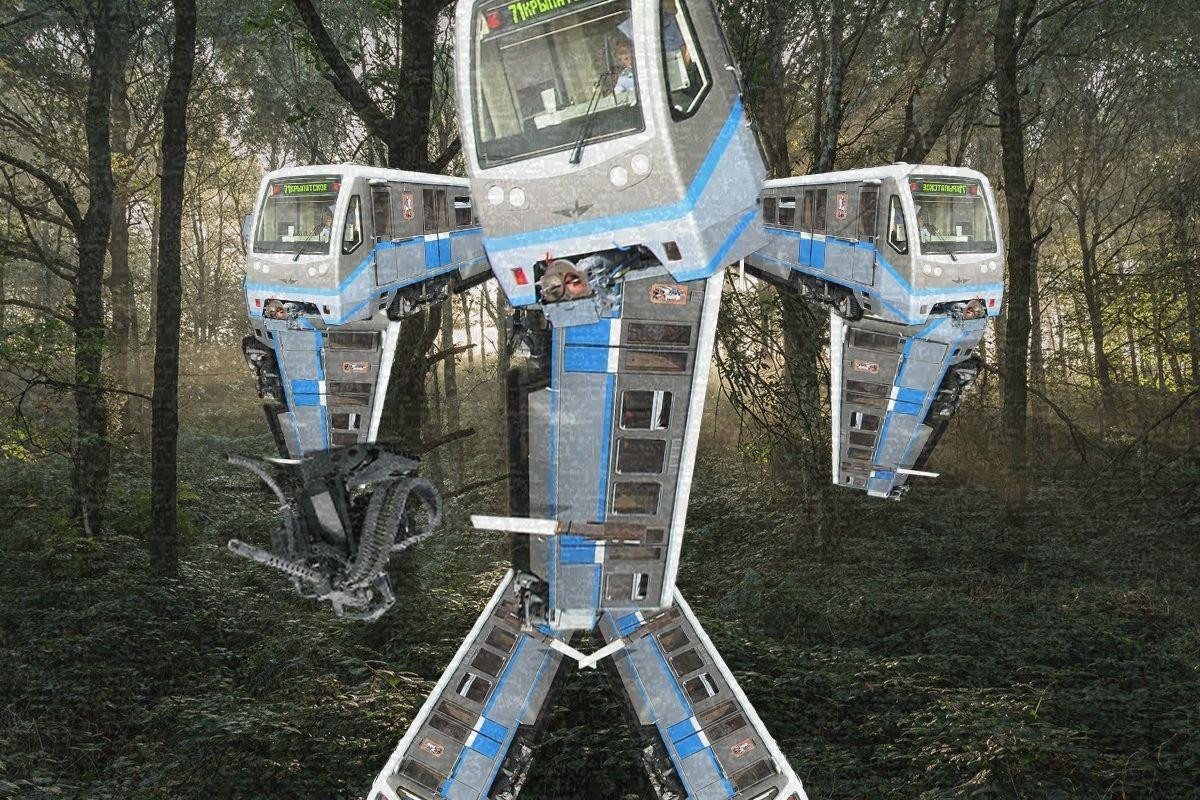
\includegraphics[width=5cm]{memes/d-meme.jpg}
  \end{center}

  \begin{itemize}
  \item Идея задачи --- Григорий Резников, МГУ
  \item Разработка задачи --- Константин Амеличев, ВШЭ
  \end{itemize}

\end{frame}

\begin{frame}{Постановка задачи}

  \begin{itemize}
  \item Дано дерево на $n$ вершинах и $m$ путей
  \item Требуется задать каждой вершине цвет $c_v$
  \item Вдоль пути цвета должны быть расположены монотонно
  \item Максимальное из чисел должно быть как можно меньше
  \end{itemize}

\end{frame}

\begin{frame}{Решение за $\O(n^n \cdot nm)$ (5 баллов)}
  \begin{itemize}
  \item Если раскраска существует, то она существует и с цветами от 1 до $n$
  \item Переберем все раскраски и проверим, что числа вдоль путей возрастают
  \end{itemize}
\end{frame}
\begin{frame}{Решение за $\O(2^n \cdot nm)$ (15 баллов)}
  \begin{itemize}
  \item Разделим ребра на покрытые и не покрытые путями
  \item Ребра второго типа разбивают задачу на несколько меньших задач
  \item Ребра первого типа задают сравнение --- либо $c_v < c_u$, либо $c_u < c_v$
  \end{itemize}
\end{frame}
\begin{frame}{Решение за $\O(2^n \cdot nm)$ (15 баллов)}
  \begin{itemize}
  \item Переберем все возможные сравнения
  \item Рассмотрим вершины в порядке топологической сортировки
  \item Задаем вершине минимальный доступный цвет
  \item Проверяем, что раскраска корректна
  \end{itemize}
\end{frame}

\begin{frame}{Граф --- звезда (10 баллов)}
  \begin{itemize}
  \item Длина каждого пути не больше 3
  \item Построим граф на путях
  \item Проведем ребро между двумя путями, если они не вложены и пересекаются
  \end{itemize}
\end{frame}

\begin{frame}{Граф --- звезда (10 баллов)}
  \begin{itemize}
  \item Выбор направления пути задает направление всей компоненте
  \item Граф должен быть двудольным!
  \item Если граф двудольный, то существует раскраска с максимальным цветом не больше 3
  \end{itemize}
\end{frame}

\begin{frame}{Пути не пересекаются, $\O(n \log C \log n)$ (10 баллов)}
  \begin{itemize}
    \item Раскраска точно существует
    \item Сделаем бинарный поиск по максимальному цвету
    \item Проверим, возможно ли раскрасить дерево в $k$ цветов
  \end{itemize}
\end{frame}

\begin{frame}{Пути не пересекаются, $\O(n \log C \log n)$ (10 баллов)}
  \begin{itemize}
    \item Динамическое программирование по поддеревьям
    \item $dp[v]$ --- минимальный возможный цвет, в который можно покрасить $v$, согласованный с поддеревом
    \item Для определенности считаем, что ребро $v \rightarrow parent_v$ направлено так, что $c_v < c_{parent_v}$
    \item В силу симметрии максимально возможный цвет, если $c_v > c_{parent_v}$ равен $k + 1 - dp[v]$
  \end{itemize}
\end{frame}

\begin{frame}{Пути не пересекаются, $\O(n \log C \log n)$ (10 баллов)}
  \begin{itemize}
    \item Для вершины $v$ есть набор ограничений
    \item Если через $v$ идет вертикальный путь из поддерева $u$, тогда $dp[v] \ge dp[u] + 1$
    \item Если через $v$ проходит путь из поддерева $a$ в поддерево $b$, тогда:
    \begin{enumerate}
        \item $dp[v] \ge dp[a] + 1$
        \item $dp[v] \le k - dp[b]$
    \end{enumerate}
    \item Но мы не знаем, в какую сторону направлен путь
  \end{itemize}
\end{frame}

\begin{frame}{Пути не пересекаются, $\O(n \log C \log n)$ (10 баллов)}
  \begin{itemize}
    \item Попробуем и так, и так
    \item $dp[v] \in [dp[a] + 1, k - dp[b]]$ или $dp[v] \in [dp[b] + 1, k - dp[a]]$
    \item Для каждого пути выпишем два отрезка, и сделаем сканлайн
    \item Найдем самую первую точку, покрытую отрезками всех цветов
    \item Решение за $\O(n \log C \log n)$
  \end{itemize}
\end{frame}

\begin{frame}{Пути не пересекаются, $\O(n \log C)$ (20 баллов)}
  \begin{itemize}
    \item Заметим, что мы взяли ограничения в два множества --- $L$ и $R$
    \item $max(L) + 1 \le min(k - R) \rightarrow max(L) + max(R) \le k - 1$
    \item $dp[v] = max(L) + 1$
    \item Надо разложить пары $dp[a_i],\,dp[b_i]$ по двум множествам
  \end{itemize}
\end{frame}

\begin{frame}{Пути не пересекаются, $\O(n \log C)$ (20 баллов)}
  \begin{itemize}
    \item Зафиксируем, что будет больше --- $max(L)$ или $max(R)$
    \item Тогда в каждой паре разложение определится однозначно --- максимум пойдет в то множество, где максимум больше
    \item Проверим оба варианта на условие $max(L) + max(R) \le k - 1$ и возьмем наилучший
  \end{itemize}
\end{frame}

\begin{frame}{Полное решение (100 баллов)}
  \begin{itemize}
    \item Как в графе-звездочке, строим новый граф
    \item Для каждого ребра становится известен класс эквивалентности
    \item Внутри классов эквивалентности мы знаем ориентацию ребер, относительно <<основного>> ребра внутри класса
  \end{itemize}
\end{frame}

\begin{frame}{Полное решение (100 баллов)}
  \begin{itemize}
    \item Бинарный поиск по ответу
    \item Аналогичная $dp[v]$
    \item Теперь вместо пары $a, b$ у нас будет два множества $A, B$. Внутри такого множества надо будет брать те $a,\,b$ что $dp[a] \ge dp[a'],\ dp[b] \ge dp[b']$.
    \item Свели к предыдущей задаче. В зависимости от подсчета динамики получаем решения за $\O(n \log C \log n)$ или $\O(n \log n)$
  \end{itemize}
\end{frame}
